\chapter{Передача інформації у часовому просторі короткоімпульсними 
електромагнітними полями}
\label{ch:neuron}

%%%%%%%%%%%%%%%%%%%%%%%%%%%%%%%%%%%%%%%%%%%%%%%%%%%%%%%%%%%%%%%%%%%%%%%%%%%%%%%
\section{Основи класичного імпульсного радіо}

Новою сферою застосування послідовної 
надширокосмугової радіоелектроніки (DS-UWB) сьогодні стає інтернет речей. 
Основними чинниками для цього стали високий рівень інформаційної безпеки, 
порівняно низький рівень споживання електроенергії та стійкість до 
вузькосмугових завад. В задачах інтернету речей, робота таких пристроїв на 
маленькій відстані є, скоріш, перевагою, а ніж недоліком через
зменшення радіо-забруднення приміщення.

Принцип роботи сучасного надширокосмугового імпульсного радіо 
послідовної передачі (без застосування стробоскопічного принципу) 
\cite{imp:ChannelImplementation} можна узагальнити наступною 
функціональною схемою (Рис.~\ref{fig:emp_radio}). Відзначимо, що згадана
схема застосується як для задач комунікації так і локації і зондування.

\begin{figure}[htbp] \begin{center}
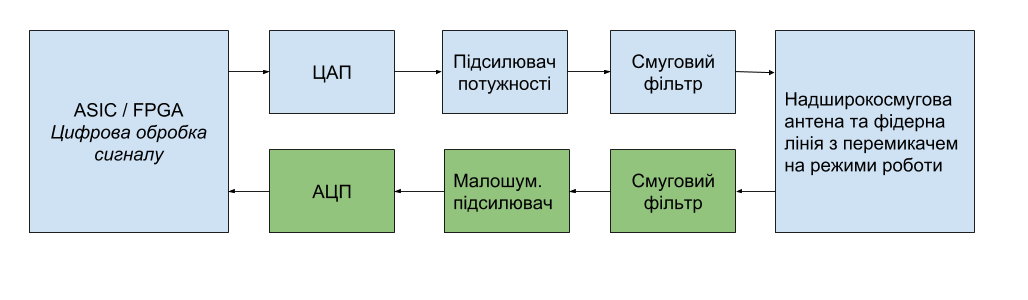
\includegraphics[scale=0.45]{classical_radio}
\caption{Класична схема імпульсного радіо} \label{fig:emp_radio}
\end{center} \end{figure}

Процес перетворення прийнятної імпульсної електромагнітної хвилі в фідерній 
системі в сигнал у дроті узагальнюють, як масштабно-часове перетворення, яке 
може бути технічно реалізовано у різний спосіб \cite{imp:Astanin1989}. 
Існуючі принципи аналогової обробки прийнятого імпульсного радіосигналу 
успадковані від схемотехніки, що використовувались для гармонійних сигналів 
\cite{imp:ComunicationsOverview}: для обробки отриманого з антени 
електричного струму використовується послідовна фільтрація та підсилення з 
подальшим оцифровуванням за допомогою АЦП і цифрової обробки в модулях 
FPGA (Рис.~\ref{fig:emp_radio}). Серед методів обробки сигналу в модулях FPGA, 
з лінійною складністю по часу можна виділити сімейство методів корелятивного 
порівняння, що базується на фільтрі Калмана. Ці методи, фактично, 
порівнюють отриманий сигнал з еталонним і надають коефіцієнт відповідності, 
чого достатньо для бінарної класифікації наявності сигналу. 

Кожен з послідовних етапів аналогової обробки, направлений на покращення 
окремої характеристики сигналу, неминуче впливає і на інші його 
характеристики, що накопичує похибку та губить частину інформації про 
сигнал та про шум:

\begin{enumerate}
	\item лінійне покращення співвідношення сигнал-шум (фільтрація), 
	на практиці, має незначний нелінійний вплив на інші характеристики НШС 
	сигналу, наприклад, крутизну імпульсу;
	\item квазі-лінійне підсилення незначним чином впливає на 
	форму імпульсу за рахунок нелінійності амплітудно-частотної 
	характеристики, а також підсилює артефакти завад;
	\item аналогово-цифрове перетворення сигналу губить частину інформації 
	про надширокосмуговий шум через дискретизацію, яка може не відповідати 
	критеріям Найквіста.
\end{enumerate}

Таким чином, на числову обробку потрапляє дещо видозміненій від початкового
сигнал. Також сам алгоритм числової обробки в модулі FPGA, зазвичай,
вибирається простим, через необхідність обробки сигналу в квазі-реальному 
часі. Крім того, використання функціональної схеми на Рис.~\ref{fig:emp_radio} 
для послідовного виокремлення корисної інформації з сигналу супроводжується
втратою можливості для врахування природи поширення імпульсних 
електромагнітних хвиль:

\begin{enumerate}
	\item в ближній зоні антени форма сигналу сильно залежить від 
	напрямку спостереження \cite{imp:Wu1985, imp:Sodin1992-10, 
	my:Telecom2018}, що призводить до зниження точності роботи радіосистем, 
	які не враховують особливості поширення хвиль, а спираються лише на 
	форму отриманих сигналів;
	\item спостерігається погіршання якості роботи радіо-обладнання через 
	невраховану нелінійну природу поширення імпульсних хвиль в просторі та в 
	компонентах антено-фідерної системи \cite{imp:BaumSSN0401}.
\end{enumerate}

Імпульсні надширокосмугові радіотехнічні пристрої мають теоретичні 
переваги над вузькосмуговими в плані інформаційної ємності 
\cite{imp:ChannelLimitations}, але на практиці, не вдається використовувати 
ці переваги повною мірою через описані складності обробки надширокосмугових 
сигналів.

%%%%%%%%%%%%%%%%%%%%%%%%%%%%%%%%%%%%%%%%%%%%%%%%%%%%%%%%%%%%%%%%%%%%%%%%%%%%%%%
\section{Імпульсний радіоприймач на базі апаратної нейронної мережі}

Всі задачі випромінювання, поширення чи дифракції хвилі формалізуються
у вигляді деяких параметричних рівнянь відносно компонентів струму чи 
компонентів поля. Коли аналітичне розв'язання такого рівняння знайти не 
вдається, а числовий метод розв'язання має значну обчислювальну складність, 
доцільно використати штучні нейронні мережі (ШНМ) прямого поширення, графові 
моделі машинного навчання або імпульсні нейронні мережі у купі з методами їх 
навчання для пошуку розв'язків.

Рівень оптимізації сучасних програмних інструментів машинного навчання, таких 
як CUDA та Tensorflow, а також рівень розвитку апаратних інструментів GPU/ASIC
дозволяють аналізувати цифрові часові послідовності за час порядку 
десятків мілісекунд, що дозволяє використовувати такі інструменти при роботі 
з сигналом у квазі-реальному часі, опрацьовуючи сигнал після АЦП. Недоліком 
такого методу може стати висока ціна кінцевих виробів, а також високий 
рівень споживання енергії. З іншого боку, галузь що швидко розвивається - 
аналогові штучні нейронні мережі виконані за технологією CMOS. На такі 
пристрої можна подати сигнал напряму з антенно-фідерної системи. Такі 
пристрої вже широко застосовуються радіотехніками в галузі когнітивного 
радіо \cite{imp:Husseini2010}, а також адаптивних вузькосмугових антенних 
систем \cite{imp:Zbynek2002}. В цих задачах, апаратні ШНМ мережі 
використовується для оптимізації деяких параметрів прийому-передачі сигналу 
в режимі реального часу.

Останнім часом, технічний розвиток в галузі апаратних штучних нейронних мереж 
дозволив втілювати їх різноманітні топологічні особливості в електронних 
аналогових пристроях. Проаналізуємо можливість застосування цих технологій для 
задач класифікації отриманого сигналу (sequence-to-label) та визначення його 
присутності в кожен момент часу (sequence-to-sequence). Результат розв'язання 
таких задач аналізу даних дозволить оцінити практичну цінність застосування 
нейронних мереж в різних задачах прикладної електродинаміки: радіолокації, 
телекомунікації, вимірювання, зондування тощо. 

Важливим напрямком розвитку CMOS технології для покращення технічних 
характеристик імпульсного радіо стає зменшення техпроцесу. Наразі існують
готові прилади CMOS LSTM з техпроцесом 180нм. Використаннм техпроцесу 5нм,
що активно розвивається, можна збільшити швидкість обробки сигналів у 
порівнянні з класичними схемами імпульсного радіо з аналогічною цифровою 
обробкою у $ 10^8 $ разів також зменшивши рівень споживання енергії.

\begin{figure}[htbp] \begin{center}
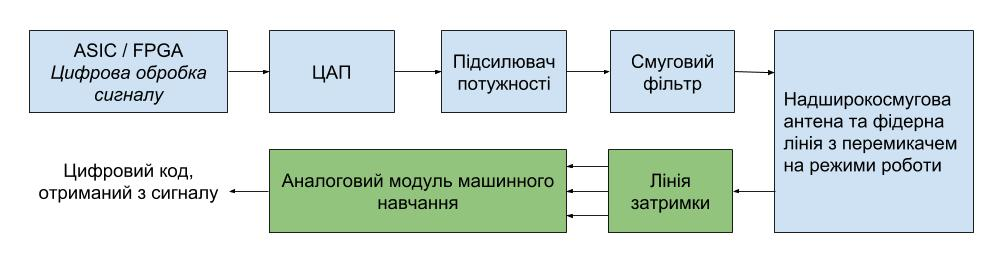
\includegraphics[scale=0.45]{neuron_radio}
\caption{Схема імпульсного радіо на нейронній схемотехніці} 
\label{fig:neural_radio}
\end{center} \end{figure}

Штучна нейронна мережа тут є електричним колом, внутрішня передавальна 
функція якого визначається лінійною комбінацією деякого набору матричних 
характеристик, які визначаються різноманітними методами оптимізації. Таким 
чином, задача обробки прийнятого радіосигналу зводиться до пошуку необхідних 
матричних параметрів. Для цього гарно підходять градієнтні методи навчання 
з учителем, де конкретна імплементація процесу тренування та набір 
тренувальних даних залежатиме від типу задачі, що розв'язується.

В якості нейронної архітектури для кіл обробки радіосигналу розглянемо
схему encoder-decoder \cite{imp:Ying2017}. 
В цій архітектурі нейронна мережа топологічно розбивається на 
дві частини. Перша частина трансформує вхідну часову послідовність в деякий 
набір параметрів, які однозначно характеризують вхідний сигнал. Тобто, 
енкодер проектує вхідний сигнал на деякий ознаковий простір. Друга частина 
мережі, декодер, перетворює набір ознак в ту якісну або кількісну 
характеристику, яку передбачає постанова задачі. Наприклад, для задачі 
телекомунікації - це інформаційне повідомлення, або для радарної 
задачі - це положення та тип цілі. Такий підхід забезпечить повторне 
використання попередньо навчених енкодерів для різноманітних задач 
радіофізики, які виконують роль врахування фізичної моделі поширення хвиль 
у вільному просторі та в антенно-фідерній системі. Технічна можливість 
додати декілька різних декодерів в електричні кола радіоприймальної схеми 
зробить цю концепцію промислово придатною.

Вихідний сигнал, що продукує апаратна нейронна мережа, визначається 
активаційною функцією вихідного нейрону. Цифровий вихідний сигнал можна 
отримати ступеневою активаційною функцією (персептрон Розенблата) та зручно 
використовувати описаний пристрій, як мереживний інтерфейс комп'ютера чи 
джерело керуючого сигналу для робототехніки.

\begin{figure}[htbp] \begin{center}
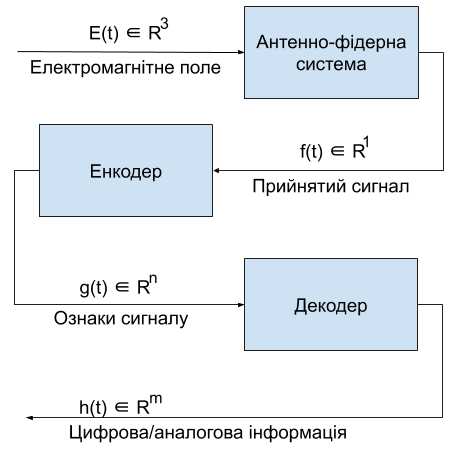
\includegraphics[scale=0.9]{DeepUWBukr}
\caption{Виокремлення корисної інформації нейронним радіо} 
\label{fig:DeepUWB}
\end{center} \end{figure}

Прикладом застосування аналогових нейронних мереж у радіо є покращення 
характеристик роботи CDMA телефонії, шляхом послідовної лінійної фільтрації
з подальшою обробкою повнозв'язною аналоговою нейронною мережею прямого 
поширення \cite{imp:Hasan2017}. Принципова відмінність нейронного
радіо від прототипу полягає у відмові від обробки кожної характеристики 
сигналу окремо, і делегації його аналізу, як цілого, пристрою, системотехніка 
якого реалізує деякий математичний граф. В досліджені \cite{imp:Zhang2009} 
задачу розрізнення збуджень різного типу виріщують за допомогою лінійного 
фільтру і, як буде показано далі, цю ж задачу краще розв'язує енкодер штучної 
нейронної мережі за рахунок врахування складної природи поширення імпульсних 
електромагнітних хвиль.

Як і класична схема імпульсного радіо, запропонована схема передбачає 
можливість застосовувати одну і ту ж антену для передачі та прийму сигналу. 
Також використання нейропроцесору не виключає застосування традиційних 
методів аналогової обробки: підсилення, фільтрація.

Важливим аспектом є те, що використання ПЗУ дозволить програмувати нейронний 
процесор шляхом встановлення нових параметрів аналогових нейронів керуючими 
напругами, що дає змогу змінювати технічні характеристики пристроїв без 
втручання в його схемотехніку. Але практика не завжди потребує такої 
гнучкості: частіше, для всього періоду використання вбудованої електроніки, 
її призначення та порядок роботи залишаються постійним, а отже керуюча 
напруга може задаватись резисторами, що значно здешевить пристрій.

Порівняння рівня споживання електроенергії аналогового нейропроцесора та 
аналогічного цифрового пристрою GPU/ASIC \cite{imp:AnalogLSTM} показало 
кращу енергоефективність для першого. Відтак, використовуючи аналогового 
нейропроцесор замість АЦП та FPGA можна скоротити споживання енергії 
надшироосмуговим радіо.

%%%%%%%%%%%%%%%%%%%%%%%%%%%%%%%%%%%%%%%%%%%%%%%%%%%%%%%%%%%%%%%%%%%%%%%%%%%%%%%
\section{Формування тренувальних даних для нейронного радіо}

Розглянемо задачу односторонньої передачі інформації через нейронне радіо. 
В якості передавальної антени розглядається антена типу LIRA. Для спрощення, 
в якості приймальної антени розглянемо ідеальний надширокосмуговий вимірювач 
напруженості електричного поля, який не змінює форму отриманого сигналу,
тобто гарантує відсутність впливу приймальної антени на форму отриманого 
сигналу. Сигнал з приймальної антено-фідерної системи подається на деяку 
апаратну нейронну мережу. Напруженість електричного поля, породженого 
випромінювальною антеною $ \vect{E}_{tx} $, можна визначити в довільній 
точці спостереження при довільному збуджені з урахуваннями ефектів ближньої 
зони, користуючись згорткою \eqref{eq:duhamel} по перехідній функції 
$ \vect{E}_0 $. Тоді, отриманий з антенно-фідерної системи сигнал, буде 
пропорційний до компонентів напруженості електричного поля випромінювальної 
антени. Здійснюючи гіпотетичне вимірювання в такій площині, що спостерігається 
$ OX $ компонента напруженості поля, а приймальна лінія ідеально узгоджена і 
немає втрат, отриманий сигнал матиме вигляд:

\begin{equation}
f_{rx} \left( \vect{r}, t \right) = 
\int_0^t \derivat{f_{tx}}{\tau} \vect{E_0} (\vect{r}, t - \tau) d \tau,
\end{equation}
%
де $ \vect{E_0} $ - перехідна функція передавальної антени типу LIRA, а 
$ f_{tx} (t) $ - форма сигналу, що збуджує передавальну антену.

Метою даного моделювання є пошук оптимальної нейронної архітектури, а також 
її вагових коефіцієнтів, що дозволить співвіднести прийнятий сигнал з деяким 
типом збудження на передавачі в умовах завад, та з урахуванням деяких ефектів 
ближньої зони.

Тренувальний набір даних для цієї задачі складатиметься з пар часових 
послідовностей - струм збудження передавальної антени $ f_{tx} (t) $ та струм, 
що буде отримано приймачем $ f_{rx} (t) $ при різних його розташуваннях 
$ \vect{r} $ відносно системи координат передавача, введеної як на 
Рис.~\ref{fig:pdisk}. Для максимально правильного функціонування мережі в 
заданих умовах, набір тренувальних даних повинен містити вичерпну інформацію про 
поведінку поля у всій області функціонування антенної системи, а тобто містити 
вимірювання в ближній і дальній зонах. Користуючись визначенням дальньої зони,
отримуємо максимальне віддалення від джерела, де необхідно проводити 
вимірювання - $ 0 \leq z \leq 8R $. Користуючись направленістю антен типу 
LIRA, обмежимо радіус поперечного зрізу циліндричної області, де проводяться 
вимірювання $ 0 \leq \rho \leq R $, а користуючись симетрією джерела розглянемо 
не весь зріз, а лише його першу чверть $ 0 \leq \varphi \leq \pi / 2 $.

Таким чином, просторовий об'єм, в якому необхідно провести вимірювання 
складає $ \pi R^2 / 2 $. З огляду на низьку сходимість деяких алгоритмів 
навчання заповнимо розглянуту область великою кількістю (10000) випадково 
розміщених і рівномірно розподілених уявних вимірювань для тренувального 
набору даних, а також в чотири рази меншим тестувальним набором - 
2500 зразків. Для наближення моделі до реальних умов до кожної
отриманої числової послідовності $ f_{rx} (t) $ додамо деяку випадкову 
заваду. Канал зв'язку з адитивним білим гаусовим шумом (AWGN або Additive 
White Gaussian Noise) -- найпростіша модель врахування завад в задачах 
комунікації, де енергія шуму визначається як квадрат середнього відхилення. 
Для оцінки зашумленості електромагнітного імпульсу вводять критерій $ SNR $ 
за децибельную шкалою:

\begin{equation} \label{eq:snr}
SNR = 10 * \log_{10} \left( \frac{W}{\sigma^2} \right),
\end{equation}
%
де $ W $ - енергія електромагнітної хвилі, а $ \sigma $ - другий статистичний 
момент моделі білого гаусівського шуму. У виразі не враховано вплив постійної 
фонової напруженості поля, яка фігурує в моделі білого шуму для каналу зв'язку 
через відсутність його впливу на часову залежність прийнятого сигналу.

\begin{figure}[htbp] \begin{center}
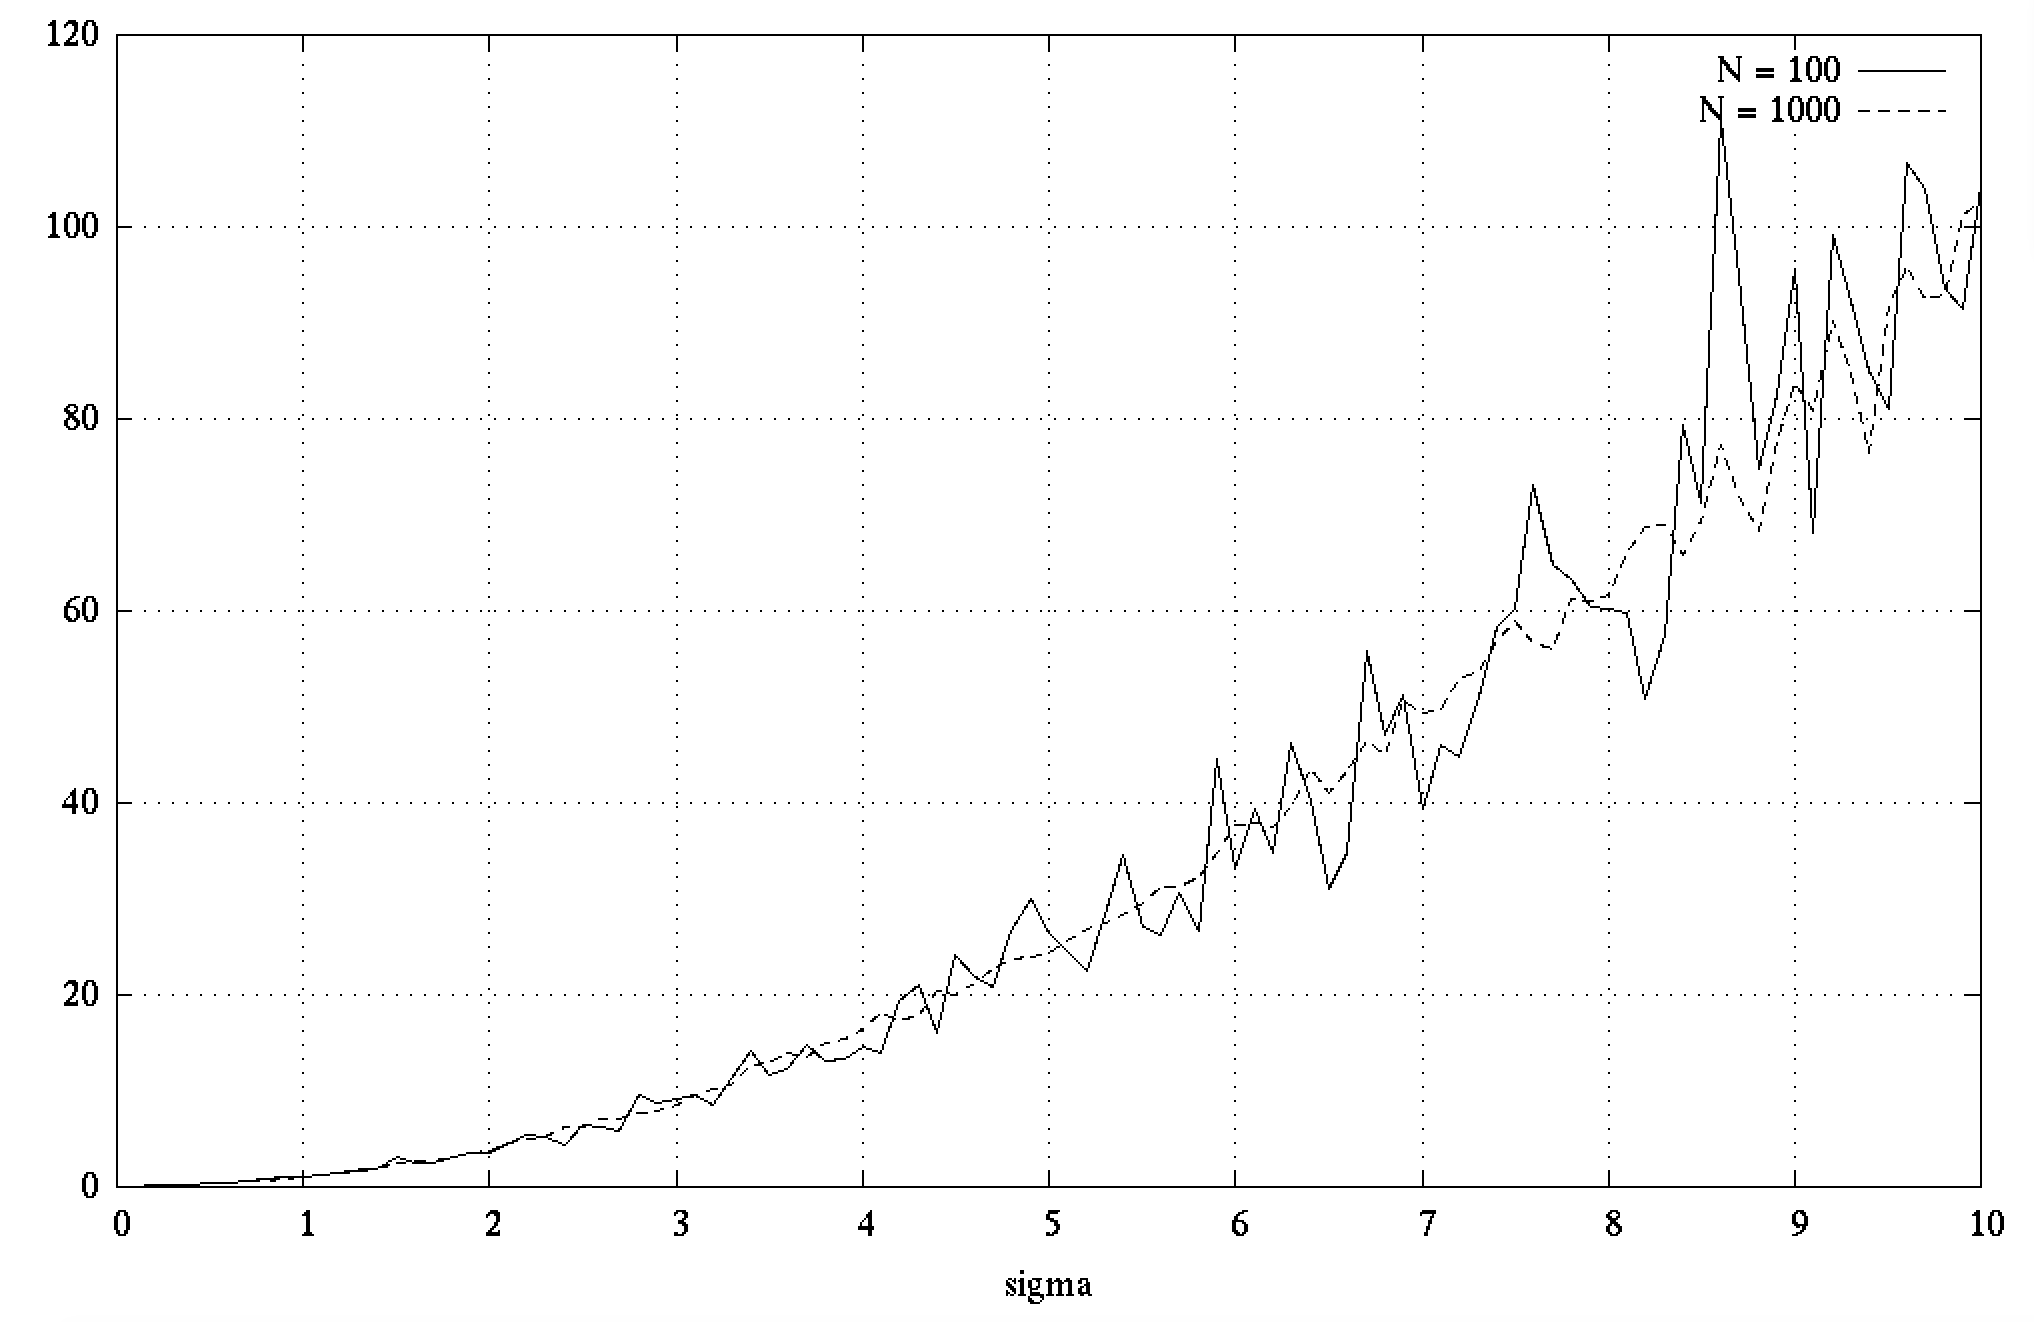
\includegraphics[scale=0.4]{P4AWGN}
\caption{Енергія моделі білого шуму в залежності від параметру} \label{fig:P4AWGN}
\end{center} \end{figure}

Через напрямлені властивості антени, навіть при постійному рівні завад, 
отриманий набір даних складатиметься зі зразків з різним значенням SNR: 
більшим на осі та меншим на периферії (Рис.~\ref{fig:SNR}), а отже постає 
питання щодо необхідної пропорційності кількостей сильно- та слабо- 
зашумлених зразків для досягнення найкращої точності моделі на реальній 
задачі. Для якісного навчання необхідно, щоб розподіл тренувальних даних за 
значенням SNR відповідав імовірнісному розподілу прийнятих сигналів за 
значенням SNR в умовах реального використання. Припустимо, що користувачі 
пристроїв будуть намагатись вести прийомо-передачу максимізуючи SNR, тоді 
реальний імовірнісний розподіл прийнятих сигналів матиме вигляд 
гаусового, через статистичні відхилення від ідеальних параметрів та в 
умовах завад.

Для якісного процесу навчання необхідно, щоб тренувальний набір даних не 
лише містив всю палітру значень SNR при кожній епосі навчання, а ще і 
послідовно зменшував його середнє значення кожного разу, досягаючи 
локального мінімуму цільової функції.

\begin{figure}[htbp] \begin{center}
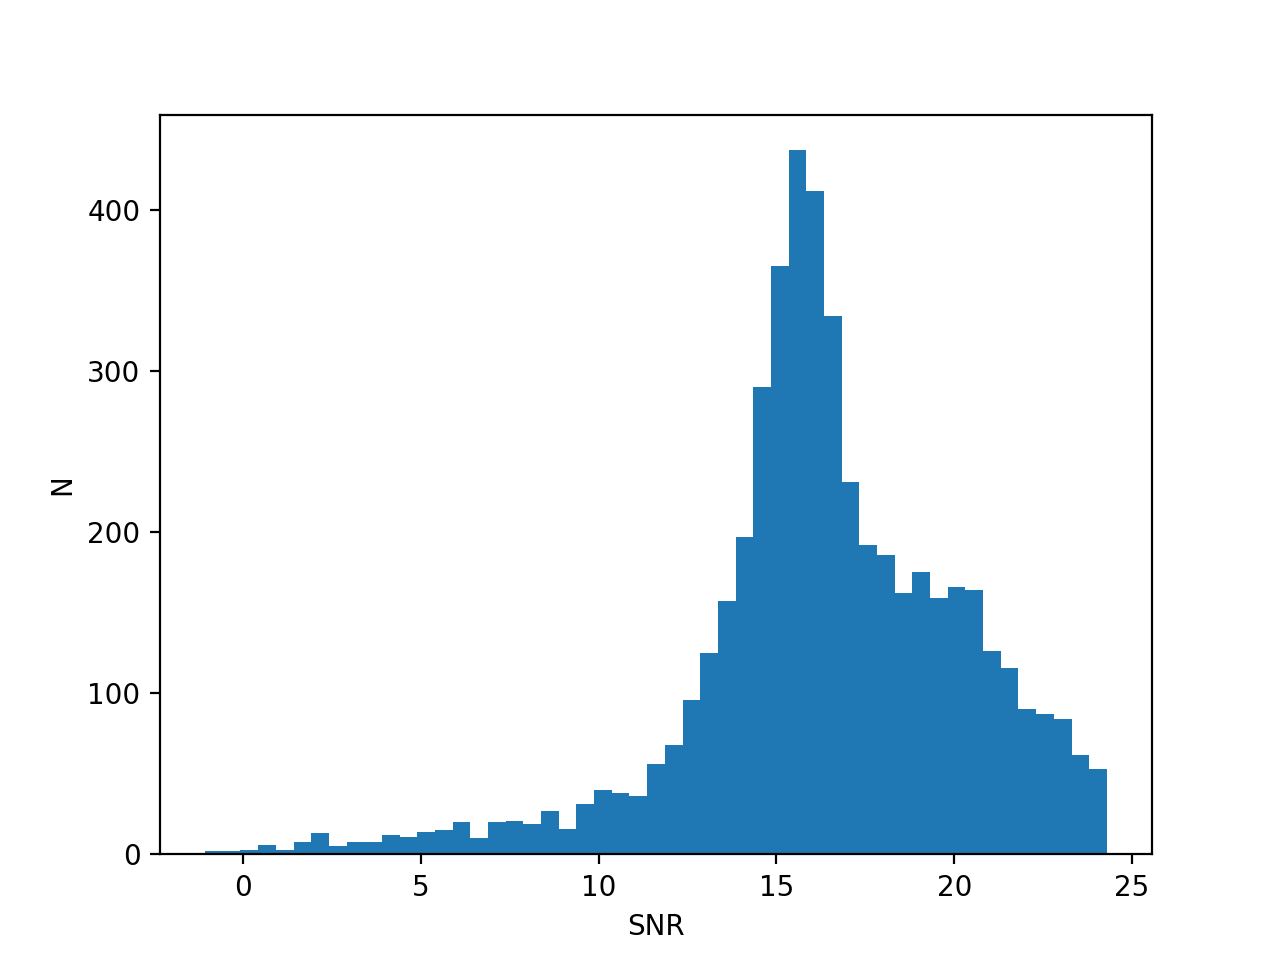
\includegraphics[scale=0.9]{Dataset_SNR}
\caption{Зашумленість набору тренувальних даних} \label{fig:SNR}
\end{center} \end{figure}

На Рис.~\ref{fig:SNR} зображено гістограму, де висота стовбчика ілюструє 
кількість зразків в датасеті з відповідним значенням SNR. Для генерації 
тренувальних даних застосовано рандомайзер mt19937 в реалізації стандартної
бібліотеки шаблонів С++ для 64-х розрядних систем за стандартом ISO C++17.

Для перевірки можливостей нейронного радіо вирізняти різні види сигналів 
розглянемо відразу декілька різних збуджувальних імпульсів $ f_{tx} (t) $:

\begin{equation} \label{eq:type_void}
f_0 = void = 0;
\end{equation}
%
\begin{equation} \label{eq:type_sinc}
f_1 = sinc = \sinc(t-\tau/2);
\end{equation}
%
\begin{equation} \label{eq:type_gauss}
f_2 = gauss = \exp(- (t-\tau/2)^2 );
\end{equation}
%
\begin{equation} \label{eq:type_gauss_perp}
f_3 = gauss\_perp = \partder{}{t} \exp(- (t-\tau/2)^2 );
\end{equation}
%
тоді отриманий набір даних матиме 4 класи, де окремим класом є клас, що 
містить лише білий шум $ f_0 $. Для дотримання збалансованості даних в 
процесі навчання, до рандомайзера додамо випадковий рівномірно розподілений 
дискретний параметр, що відповідатиме за тип збудження: \textit{void}, 
\textit{sinc}, \textit{gauss}, \textit{gauss\_perp}. Для максимізації 
якості навчання розглянемо лише датасет, де вибірки за типом збудження 
будуть кількісно збалансовані. 

Процес навчання штучної нейронної мережі може проходити як на комп'ютері так 
і на апаратному модулі за рахунок створення спеціальних програмних драйверів
до апаратної частини. В межах даного дослідження достатньо навчання на 
комп'ютері, як на ресурсах CPU так і на ресурсах GPU. Для цього набір 
тренувальних даних необхідно дискретизувати. Частоту дискретизації 
вибираємо, користуючись критерієм Найквіста.

Тобто кожен зразок тренувального набору складатиметься з часової
послідовності, що відповідає прийнятому сигналу та метаданих, що описують 
тренувальний зразок: значення енергетичного SNR, тип збудження, 
точка спостереження, ефективна тривалість збудження та інше. Для цього
зручно використати формати зберігання даних JSON та TFRecord.

%%%%%%%%%%%%%%%%%%%%%%%%%%%%%%%%%%%%%%%%%%%%%%%%%%%%%%%%%%%%%%%%%%%%%%%%%%%%%%%
\section{Моделювання демодуляції імпульсних сигналів повнозв'язною фізичною нейронною мережею}

Розглянемо декілька моделей нейронних мереж та визначимо недоліки та переваги
кожної з них. Сімейство моделей, що розглядається звузимо лише до тих, які 
придатні до виготовлення у вигляді електричних ланцюгів. Перші моделі штучних 
нейронних мереж прямого поширення, що були винайдені - повнозв'язні з одним 
прихованим шаром.



\begin{figure}[htbp] \begin{center}
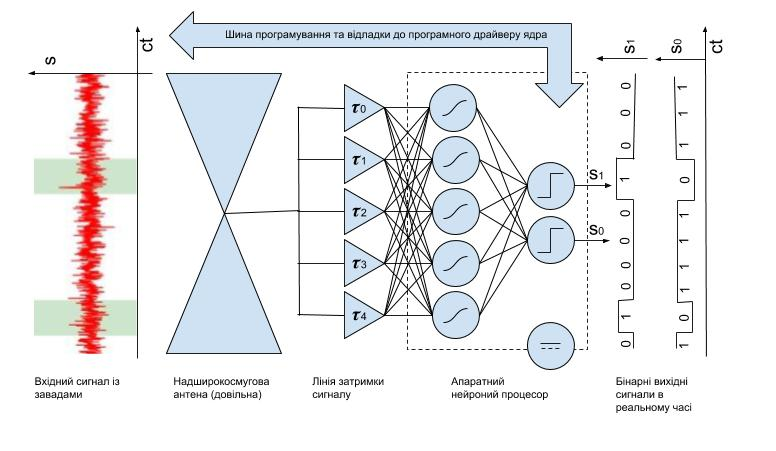
\includegraphics[scale=0.65]{simple_radio}
\caption{Імпульсне радіо на основі багатошарового перцептрону} 
\label{fig:mp_radio}
\end{center} \end{figure}

Такі мережі є популярним інструментом розв'язання задач різного типу 
\cite{imp:Kussul2004}, в основному, через досить простий алгоритм навчання.
Для подачі часової послідовності (сигналу) на її вхід обов'язковим стає 
застосування методики ковзного вікна за допомогою ліній затримки, що 
призводить до втрати частини даних. Такий підхід забезпечує подачу до 
нейронної мережі ковзного вікна даних та не враховує результат обробки 
минулого вікна при переході до наступного.

Розмірність вхідного шару визначається частотою дискретизації та мінімально 
допустимою шириною ковзного вікна, яка цілковито вміщує в себе сигнал. Для 
імпульсів, переданих антеною типу LIRA з одиничним електричним розміром, 
вхідний шар складатиметься не менше ніж з 300 штучних нейронів.

Останній вихідний шар виконує функцію декодеру і має розмірність 
якісної або кількісної характеристики, яку передбачає постанова задачі.
У випадку, що розглядається, шукана якісна характеристика -- це тип 
збудження, який може приймати чотири дискретні значення. Таким чином,
розмірність вихідного шару -- 4.

% Так як сигнал може 
% знаходитись в будь-якій частині вікна прихований шар повинен містити не 
% меншу кількість нейронів для збереження якісного результату в кожен момент 
% часу. З іншого боку, для більшості задач електродинаміки важливо визначити, 
% що сигнал взагалі був в якомусь з вікон,
% що накладаються, тому кількість нейронів в другому шарі можна дещо зменшити.

Кількість штучних нейронів у другому (прихованому) шарі повнозв'язних 
ШНМ, зазвичай, встановлюють меншою за кількість нейронів вхідного шару 
(300 нейронів) та більшою за кількість нейронів вихідного шару (4 нейрони).
Оптимальну кількість нейронів, здебільшого, визначають експериментально.
Зробивши прихований шар меншим за потрібне -- отримаємо недостатню 
запам'ятовувальну здатність нейронної мережі, в іншому випадку алгоритм 
навчання може стати нестабільним та більш тривалим. З огляду на те, що
більша кількість нейронів надмірно не вплине на якість результату, 
встановимо заздалегідь завищену кількість нейронів прихованого шару -- 
150 штук.

Так як ШНМ має три послідовні шари, що складаються з 300, 150 та 4 нейронів 
відповідно, кількість параметрів мережі, що підлягають тренуванню -- 
$ 45754 $. Для розв'язання електромагнітних задач на кшталт зондування, де 
необхідно враховувати перевідбиття сигналу, розмір вікна значно збільшиться, 
що призведе до зростання кількості тренувальних параметрів до величини 
порядку $ 10^7 $.

\begin{figure}[htbp] \begin{center}
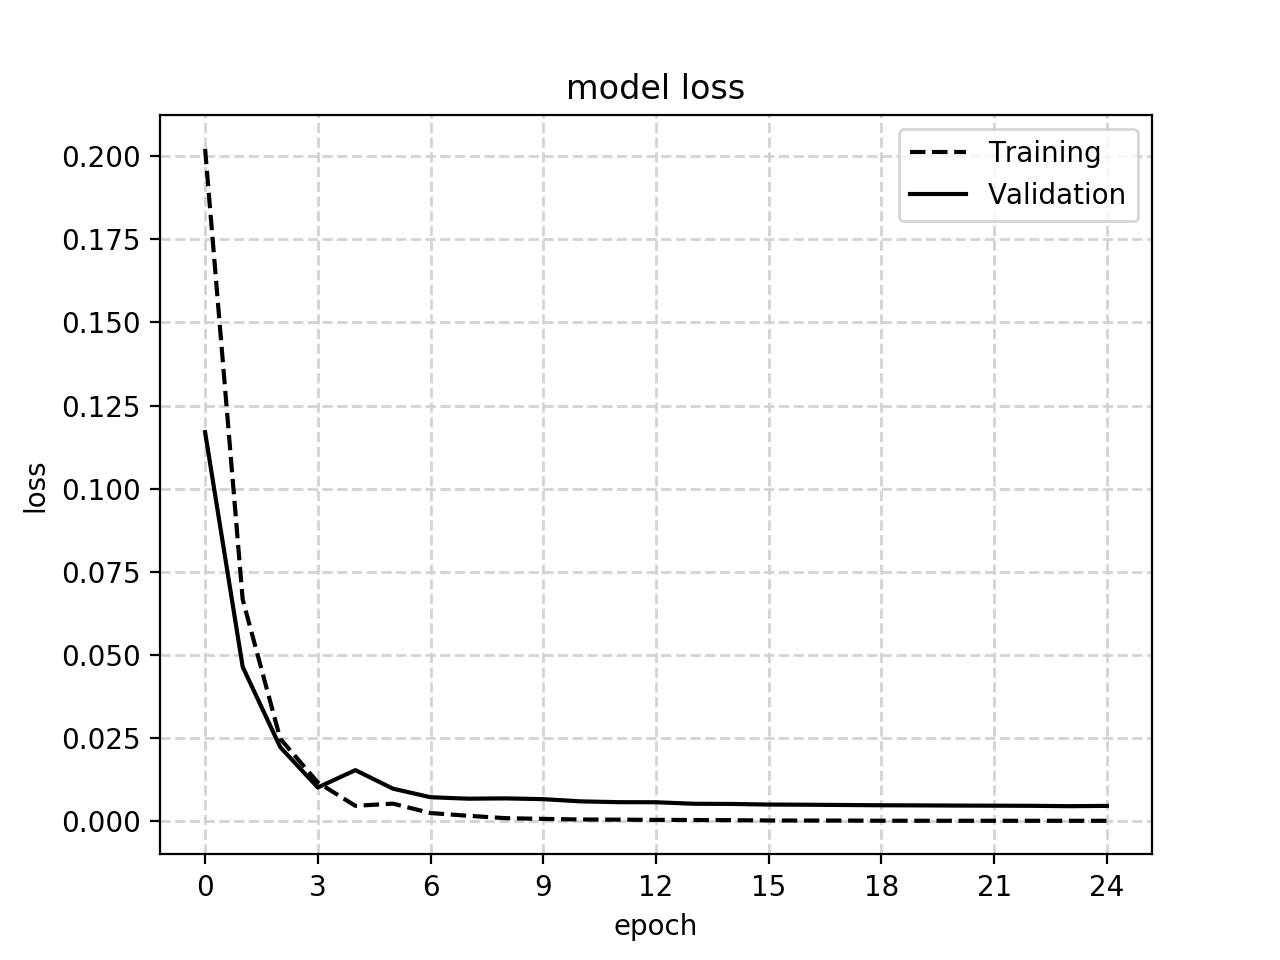
\includegraphics[scale=0.80]{FC_S2L_loss}
\caption{Зміна значення цільової функції повнозв'язної моделі  
в процесі тренування} \label{fig:fcnn_loss}
\end{center} \end{figure}

Не дивлячись на величезну кількість тренувальних параметрів, навчання 
проходить досить швидко за рахунок малої глибини моделі. 
На Рис.~\ref{fig:fcnn_loss} зображено зміну значень цільової функції в 
процесі тренування. Її пораховано на тренувальних і на тестувальних даних 
та зображено окремими кривими. Перетин тренувальної та тестувальної 
цільової функції після третьої епохи є індикатором перенавчання моделі. 
Для тренування використовувалась техніка Dropeout (виключення окремих 
нейронв з деяких етапів навчання), що в купі з перенавчанням вказує
на недостатню інформаційну ємність повнозв'язної моделі для 
розв'язання поставленої задачі.

Задачею радіоприймача є перетворення в реальному часі сигналу з антени в 
деяку послідовність корисних даних. Згідно класифікації задач аналізу даних, 
цю задачу можна розглядати як many-to-many так і many-to-one. Повнозв'язна 
нейронна мережа працює саме за схемою many-to-one, коли деякому вікну, що 
спостерігається, призначається одна якісна характеристика -- вектор 
імовірностей присутності сигналів кожного з видів.

Точність роботи, визначена за метрикою середньої відносної помилки, яка
має сенс лише до третьої епохи, через проблему перенавчання, що наступає 
коли криві перетинаються. Таким чином, мінімальне значення середньої 
відносної помилки для штучної нейронної мережі пов'язаного типу складе 
$ 89 \% $.

Серед недоліків застосування описаної архітектури в якості нейронного радіо
можна відмітити велику кількість тренувальних параметрів, що ускладнить 
електронну схему пристрою. Цю проблему можна вирішити використанням 
рекурентних штучних нейронних мереж, які одномоментно приймають на вхід 
одне значення часової послідовності і накопичують інформацію про сигнал 
з плином часу за рахунок зміни свого внутрішнього стану.

%%%%%%%%%%%%%%%%%%%%%%%%%%%%%%%%%%%%%%%%%%%%%%%%%%%%%%%%%%%%%%%%%%%%%%%%%%%%%%%
\section{Моделювання демодуляції сигналу фізичною рекурентною 
	нейронною мережею}

На відміну від повнозв'язної моделі, рекурентні можуть працювати як за схемою
many-to-one так і за схемою many-to-many, коли вхідний сигнал в кожен момент 
часу описується затребуваною якісною або кількісною характеристикою.

У випадку many-to-one прогноз нейронної мережі стосується ковзного 
вікна в цілому, а отже, точність визначення меж сигналу у часі буде визначена 
розміром вікна спостереження, яке в декілька разів ширше за сигнал. Моделі, 
що працюють за схемою many-to-many позбавлені цього недоліку і за рахунок 
наявності оцінки сигналу в кожен момент часу надають чітку межі присутності
імпульсу у деякому сигналі. 

Так як режим роботи нейронної мережі, а тобто many-to-one або many-to-many,
визначається алгоритмом тренування, апаратна реалізація пристрою залишається 
однаковою для many-to-one і many-to-many схем, що зручно для прикладного 
застосування.

Основним недоліком класичної рекурентної ШНМ є нестабільність процесу 
навчання -- проблеми exploding gradient і vanishing gradient. Саме для 
вирішення цих проблем були створені рекурентні мережі з більш складним 
зворотнім зв'язком GRU та LSTM \cite{imp:Hochreiter1997}.

\begin{figure}[htbp] \begin{center}
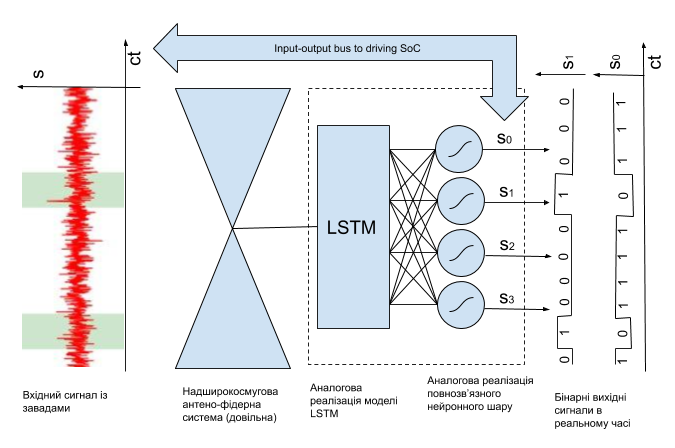
\includegraphics[scale=0.6]{lstm_radio}
\caption{Імпульсне радіо на основі нейронної мережі 
довго-короткотривалої пам'яті} \label{fig:lstm_radio}
\end{center} \end{figure}

На Рис.~\ref{fig:lstm_radio} зображено нейронне радіо з використанням 
рекурентних штучних нейронних мереж. Вихідний шар (декодер) залишився без 
змін - його розмірність визначається практичними потребами. В поточному 
досліді нейрони останнього шару мають сигмоїдальні активаційні функції 
та відповідають імовірностям спостерігати сигнал певного типу. Вхідний 
шар ШНМ є рекурентним, тобто закладається з ланцюжку однакових нейронів.
Описана штучна нейронна мережа має лише 38-116 змінних параметрів в 
залежності від типу рекурентного шару.

Розглянемо в якості вхідного шару LSTM ланцюжок. Його перевага над 
GRU в контексті нейронного радіо -- універсальність: він працює як за схемою
many-to-one так і за схемою many-to-many. Єдиним недоліком LSTM у порівнянні 
з GRU топологією стане більш тривале поширення сигналу крізь такий шар,
що можна нівелювати, використовуючи менший техпроцес.

Спершу розглянемо якість роботи рекурентної аналогової штучної нейронної 
мережі режим роботи many-to-one, щоб порівняти результат з повнозв'язаною 
нейронною мережею.

\begin{figure}[htbp] \begin{center}
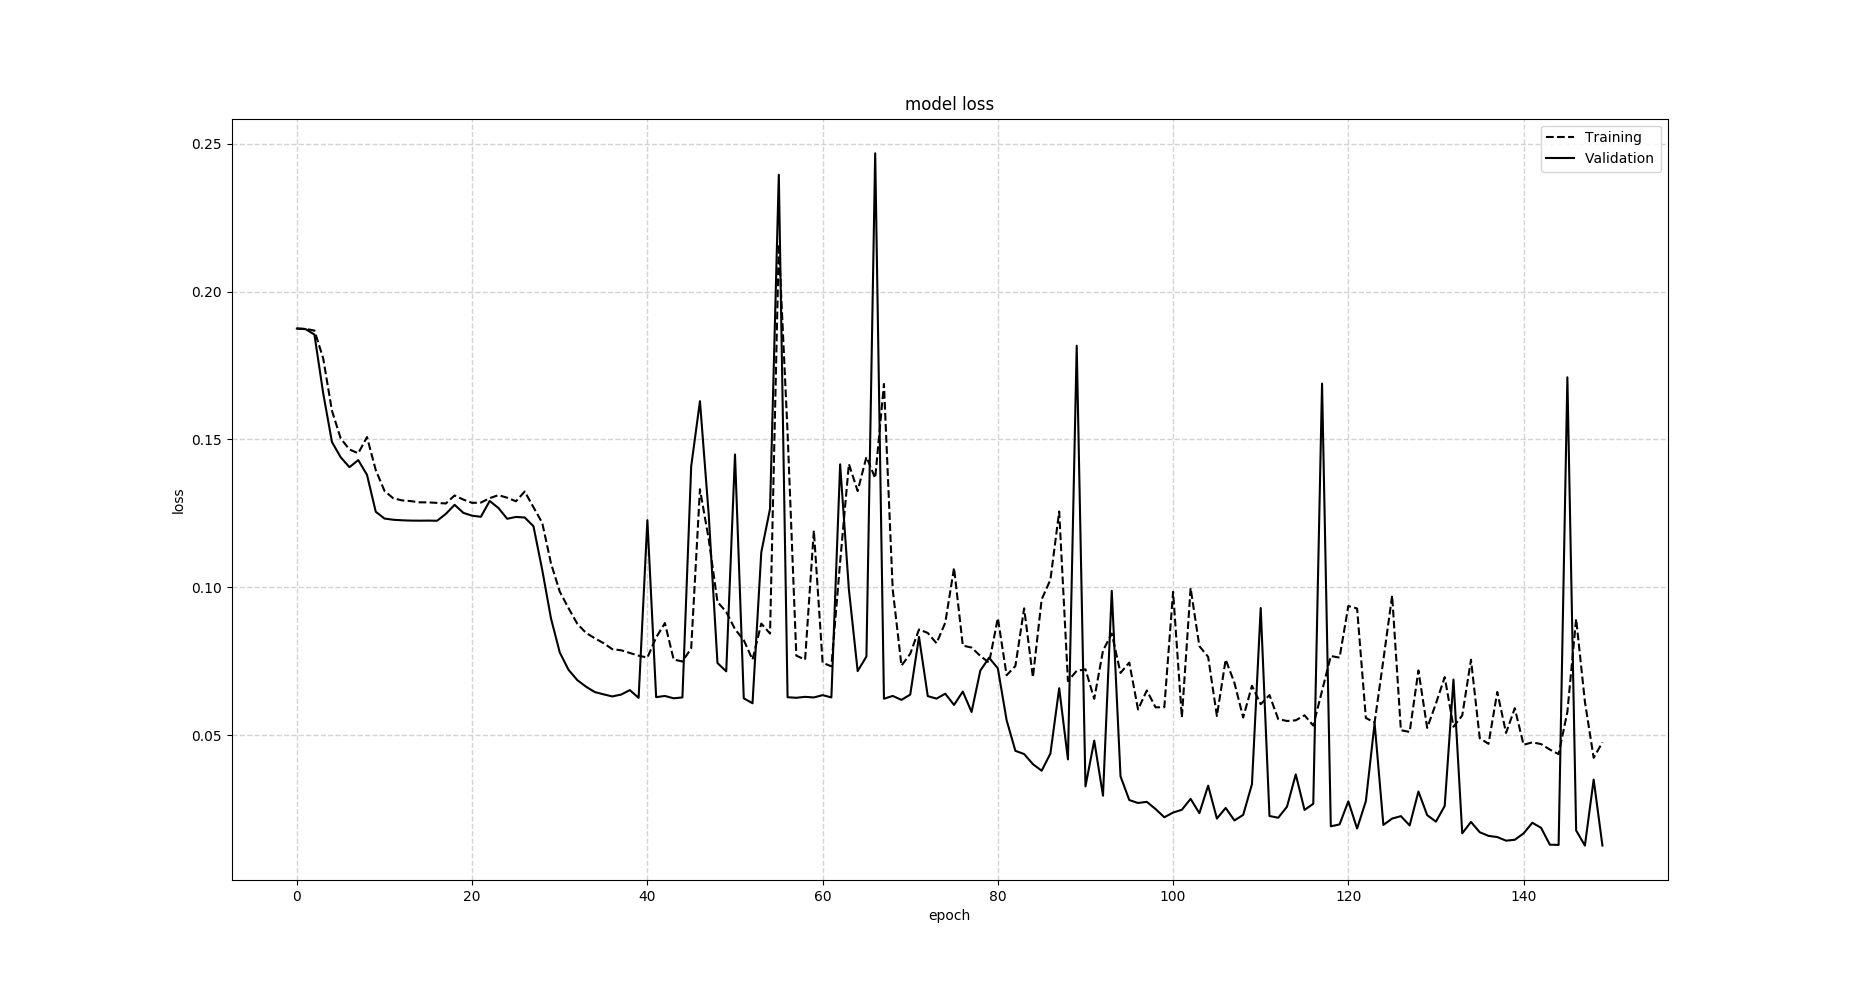
\includegraphics[scale=0.35]{LSTM_S2L_loss}
\caption{Зміна значення цільової функції моделі LSTM 
в процесі тренування} \label{fig:lstm_loss}
\end{center} \end{figure}

На Рис.~\ref{fig:lstm_loss} зображено зміну значень цільової функції в процесі
навчання. Помічаємо, що швидкість навчання 
не рівномірна -- спостерігаються ``плато'' зі сталими значеннями цільової 
функції за виключенням випадкових викидів. Подальший аналіз показав, 
що кожен з таких відрізків відповідає за навчання розпізнаванню кожного з 
типу сигналів, що вивчаються. Як можна помітити на Рис.~\ref{fig:lstm_loss},
кожен наступний тип сигналу вивчається довше попереднього. Порядок вивчення 
імпульсів теж виявився не випадковим: чим ширший спектр має імпульс, тим  
пізніше починається і довше триває його запам'ятовування.

Бачимо, що застосування нейронних мереж замість лінійної фільтрації 
дозволяє здійснювати класифікацію імпульсів у ближній зоні антени, де 
форма сигналу досить мінлива \cite{my:UWBUSIS2018}.

Використовуючи рекурентні нейронні мережі, натреновані за схемою many-to-one, 
можна досягти точності в $ 99.7\% $, що значно перевищує результати 
повнозв'язної нейронної мережі. Однак, з Рис.~\ref{fig:lstm_loss} видно, що 
використання рекурентних нейронних мереж помітно сповільнює процес навчання: 
кількість епох тренування зросла на два порядки.

Тепер розглянемо тренування за моделлю many-to-many. Топологія мережі 
залишається як на Рис.~\ref{fig:lstm_radio}, а дані для тренування
заанотуємо в кожен момент часу окремо, замість анотування даних для вікна 
спостереження.

\begin{figure}[htbp] \begin{center}
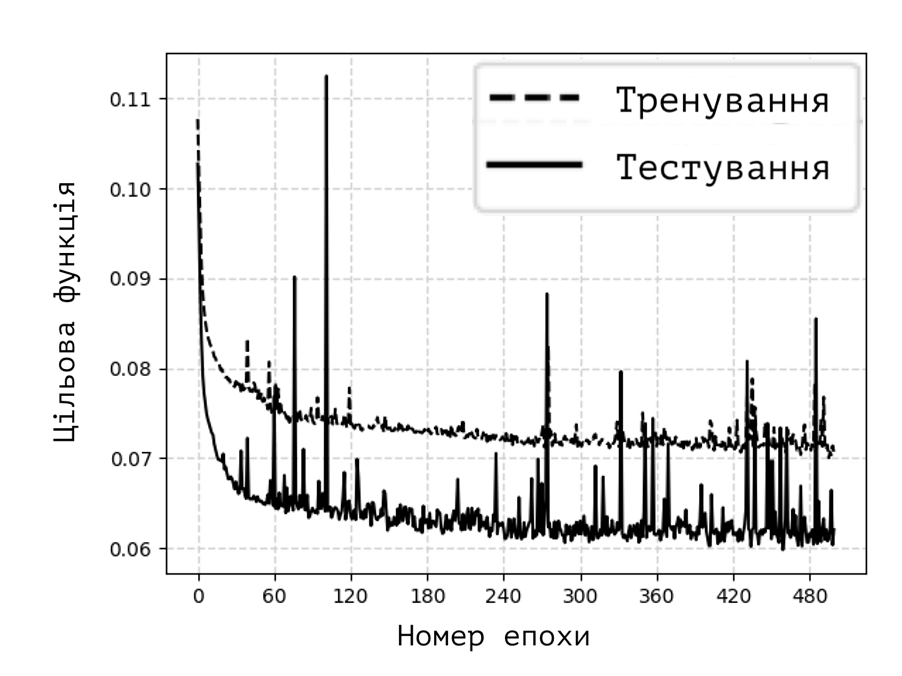
\includegraphics[scale=0.8]{lstm-seq2seq-loss}
\caption{Зміна значення цільової функції моделі LSTM
в процессі тренування} \label{fig:lstm_seq2seq_loss}
\end{center} \end{figure}

На Рис.~\ref{fig:lstm_seq2seq_loss} зображено зміну значень цільової функції
в процесі тренування нейронної мережі з Рис.~\ref{fig:lstm_radio} для 
розв'язання задачі маркування послідовності (many-to-many). Мінімальне значення 
цільової функції дозволить максимізувати здатність моделі визначати
імовірність присутності сигналу певного виду в певний момент спостереження.
При переході від many-to-one до many-to-many тренування помітно сповільнилось.

\begin{figure}[htbp] \begin{center}
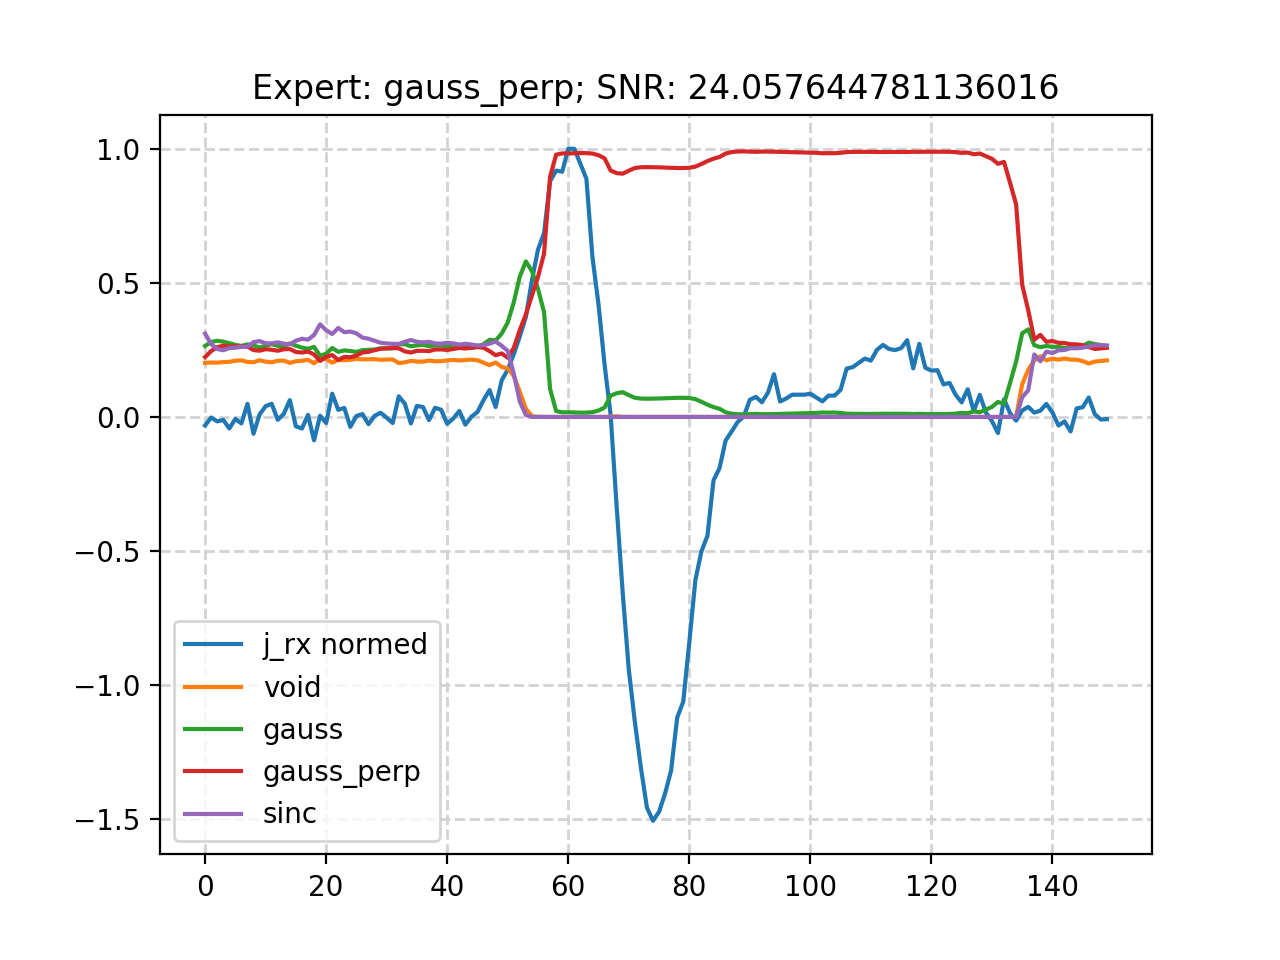
\includegraphics[scale=0.9]{seq2seq_example}
\caption{Приклад правильного аналізу} \label{fig:seq2seq_example}
\end{center} \end{figure}

На Рис.~\ref{fig:seq2seq_example} зображено приклад роботи рекурентної 
штучної нейронної мережі для класифікації прийнятого надширокосмугового сигналу 
в кожен момент часу. В представленому зразку даних спостерігається сигнал,
породжений збудженням антени типу LIRA, що має часову залежність у вигляді 
похідної від гаусіна \eqref{eq:type_gauss_perp} та спостерігається з 
таким відхиленням від осі $ OZ $, що збуджене поле виглядає як поле породжене 
збудженням з чсовою залежністю у вигяді функції Гауса \eqref{eq:type_gauss}. 
Також на рисунку зображені імовірності приналежності сигналу в кожен момент 
часу до певного типу \eqref{eq:type_void} -- \eqref{eq:type_gauss_perp}.

Для проміжку часу, що передує видимому імпульсу імовірності приналежності 
сигналу до одного з типів залишаються 
приблизно рівними та складають близько $ 25 \% $. Тобто при спостеріганні 
білого шуму значення виходу нейронної мережі, фактично, не правильне. Не 
дивлячись на це, наявність сигналу можна визначити, аналізуючи всі вихідні 
значення ШНМ: якщо імовірності наявності сигналів кожного з типів (в тому 
числі і його відсутності) рівні, то спостерігається лише шум і цю системн 
похибку можна врахувати. Таку похибку можна пояснити тим, що нейронна мережа 
намагається виокремити в шумі сигнал кожної з вивчених форм, а не знайшовши 
сигналу повертає мінімальний рівноімовірний результат.

На Рис.~\ref{fig:lstm_seq2seq_loss} проілюстровано, що навіть у ближній зоні, 
де форма імпульсу може змінюватись настільки, що стає більше схожою на інший 
сигнал, нейронне радіо гарантує стійкий режим роботи. З моменту, коли сигнал 
візуально спостерігається (індекси часової послідовності 
$ \left[ 45, 55 \right]$ ), деякий час імовірність приналежності сигналу до 
деяких типів зростає одночасно. Це можна пояснити через схожість 
градієнта часової послідовності на градієнта сигналів різних типів. Далі,
значення імовірностей стабілізуються на весь час тривалості сигналу.

Точність роботи мережі на валідаційному датасеті впала до $ 98.9\% $,
що є закономірним при підвищенні точності визначення тривалості сигналу.

\begin{figure}[htbp] \begin{center}
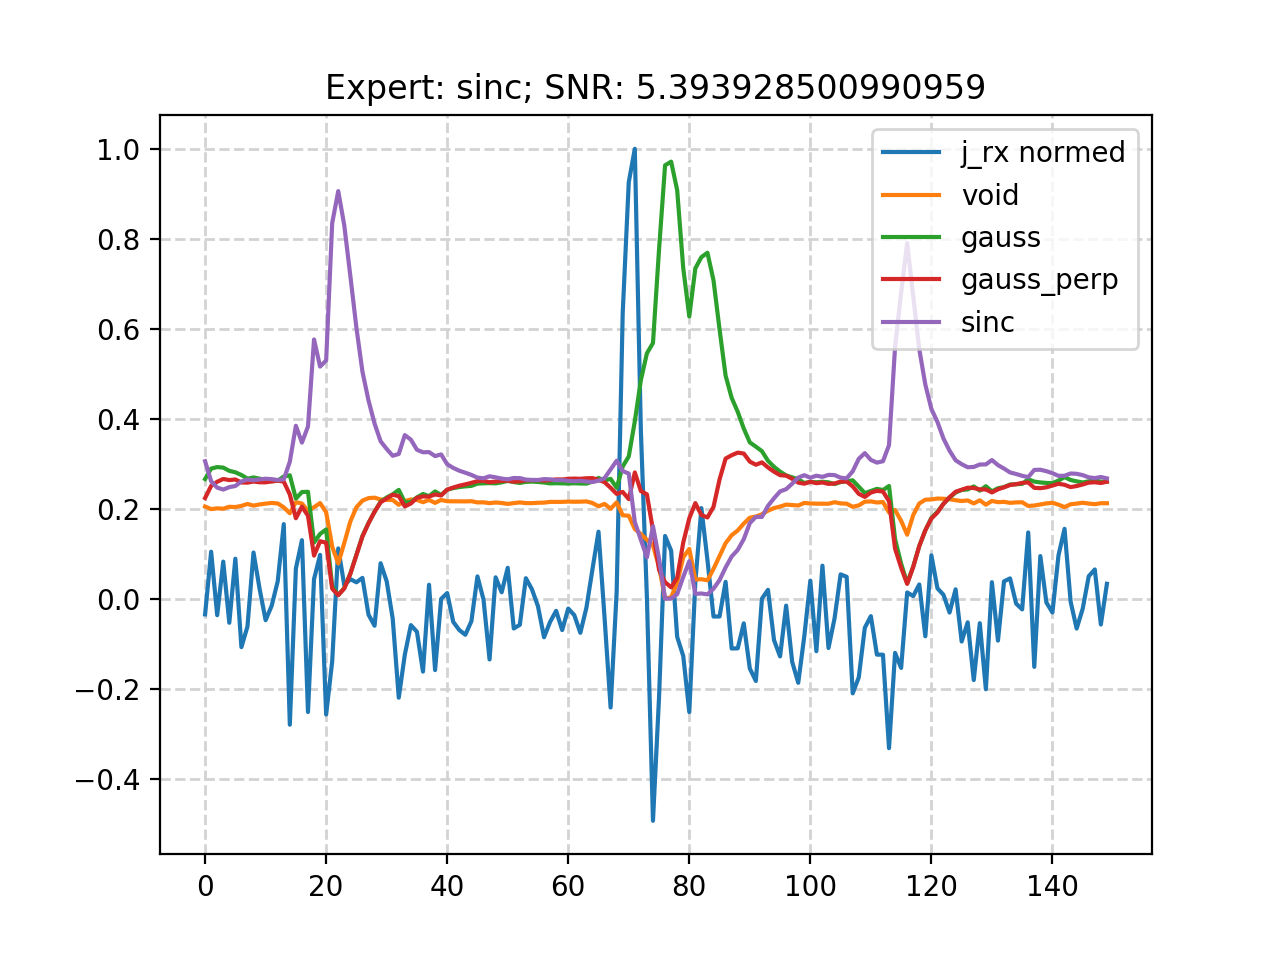
\includegraphics[scale=0.9]{lstm_seq2seq_bad}
\caption{Приклад неправильного аналізу} \label{fig:lstm_seq2seq_bad}
\end{center} \end{figure}

На Рис.~\ref{fig:lstm_seq2seq_bad} зображено приклад неправильного
розпізнавання сигналу. Зразок містить сигнал, породжений збудженням антени 
типу LIRA, що має часову залежність у вигляді \eqref{eq:type_sinc}. 
Рекурентна штучна нейронна мережа надала нестійку
детекцію трьох сигналів в хронологічній послідовності: \textit{sinc}, 
\textit{gauss}, \textit{sinc}. Детекція першого сигналу викликана 
одномоментною схожістю сигналу на \textit{sinc}, що викликало ланцюжкову 
реакцію для подальших помилкових детекції сигналів: мережа гадає, що 
помилково детектований сигнал накладається на реальний сигнал і робить 
невірне передбачення класу його приналежності.

% \begin{figure}[htbp] \begin{center}
% 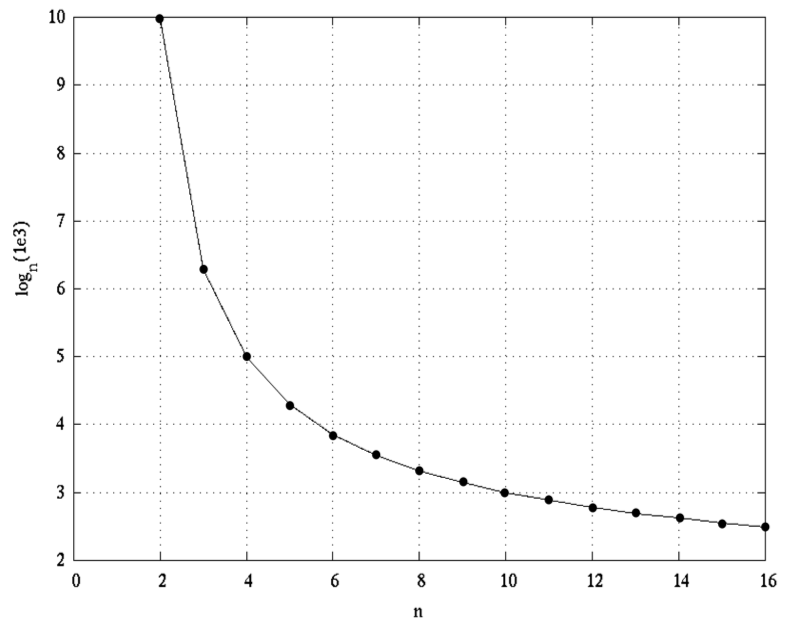
\includegraphics[scale=0.7]{channel_capacity}
% \caption{Інформаційна ємність імпульсного випромінювання} \label{fig:info_cap}
% \end{center} \end{figure}

%%%%%%%%%%%%%%%%%%%%%%%%%%%%%%%%%%%%%%%%%%%%%%%%%%%%%%%%%%%%%%%%%%%%%%%%%%%%%%%
\section{Топологія нейронного радіо та її застосування}

Як було показано, застосування аналогової повнозв'язної штучної нейронної 
мережі прямого поширення дозволяє виокремлювати інформацію з отриманих 
електромагнітних хвиль, покращуючи якісні характеристики приймача у 
порівнянні з класичним імпульсним радіо. Застосування енкодеру у вигляді 
рекурентної нейронної мережі робить нейронне радіо придатним для практичної 
реалізації через суттєве зменшення кількості штучних нейронів, а також 
покращить якість роботи, за рахунок топологічного врахування принципу 
причинності і принципу суперпозиції.

Для первинного навчання нейронного радіо застосовуються дані, отримані 
теоретичним моделюванням, замість експериментальних вимірювань задля спрощення 
промислового виробництва пристроїв. При такому підході,
різниця реальних даних і тренувальних викликає падіння точності детектування.
Шляхом вирішення цієї проблеми є застосування методів перенесення навчання, які 
широко використовуються в задачах аналізу часових послідовностей. 

Сутність методів перенесення навчання полягає в дотренуванні окремих елементів 
мережі, користуючись експериментально отриманими даними, для адаптації її 
параметрів для реальних умов. Таким чином, первинне тренування на даних,
отриманих моделюванням, дозволяє суттєво зменшити об'єм необхідних 
емпіричних вимірювань \cite{imp:Bozinovski2020}.

Також варто розглянути графічний шар в якості декодеру, що використовують в
задачах аналізу розпізнавання усної мови на кшталт розпізнавання голосових 
команд або в задачах аналізу даних з сенсорів
присутності людини в приміщенні. Схожість даних
тренування в задачах розпізнавання звуків та усної мови робить перспективним
дослідження рекурентно-графічних архітектур також в задачах комунікації, де 
для кодування використовуються імпульси різної форми (high radix networking
або multiuser enviroment).
Крім того, перспективним напрямком розвитку методики є застосування 
імпульсних фізичних нейронних мереж.

Користуючись формулою Шенона для надширокосмугових систем 
\cite{imp:ChannelLimitations} можна оцінити перспективність кодування 
інформації великою кількістю імпульсів різної форми та тривалості:

\begin{equation}
C = \frac{1}{N_{smp}} 
\frac{\log_{N_{smp}} \left( 1 + SNR \right)}{1/B + \tau_{RMS}},
\end{equation}
%
де $ C $ -- інформаційна ємність, $ N_{smp} $ -- кількість доступних 
імпульсів різної форми та тривалості (радікс), $ B $ -- ширина спектру, 
$ \tau_{RMS} $ -- скважність, а $ SNR $ -- співвідношення сигнал-шум.
Аналізуючи залежність між кількістю імпульсів та інформаційною ємністю, 
можемо зробити висновок, що збільшення $ N_{smp} $ зі класичних двох до 
шести збільшить кількість інформації в три рази.

% Для налагодження якісного імпульсного зв'язку використовують послідовності 
% імпульсів для кодування одного біту, що дозволяє розв'язати задачу 
% імпульсної комунікації в умовах перевідбиттів (multipath problem).

% При використанні запропонованої рекурентно-графічної моделі, графічний 
% декодер не вирішує проблему перевідбиттів (multipath): недостатня 
% запам'ятовувальна здатність графічної моделі призводить до лінійного 
% погіршення якості детектування імпульсу при кількісному збільшенні імпульсів, 
% що кодують сигнал. Очевидно, що топологічне ускладнення декодеру, наприклад 
% застосування LSTM, дозволить вирішити цю проблему. З іншого боку, замість 
% ускладнення декодеру, простіше застосувати FPGA для аналізу цифрового сигналу, 
% що повертається нейронним радіо.

При розв'язанні задач зондування, де інформація про об'єкт зондування 
прихована у відбитих після-імпульсних коливаннях, тривалість яких фактично 
нескінченна, виникає необхідність обмеження максимальної глибини зондування 
при використанні класичної схеми прийму (Рис.~\ref{fig:emp_radio}).
Нейронне радіо з рекурентним енкодером позбавлене цього недоліку, проте, з 
огляду на обмеженість запам'ятовувальної здатності LSTM ланцюга,
заглиблення цілі призводить до втрати точності розпізнавання. Аналогічний 
недолік рекурентних мереж може проявитись в умовах перевідбиттів (multipath 
problem) в задачах комунікації. Серед методів, які дозволяють збільшити 
запам'ятовувальну здатність енкодеру: Bi-LSTM, LSTM-to-LSTM при 
many-to-many зв'язками та Attention based LSTM.

%%%%%%%%%%%%%%%%%%%%%%%%%%%%%%%%%%%%%%%%%%%%%%%%%%%%%%%%%%%%%%%%%%%%%%%%%%%%%%
\section*{Висновки до розділу \ref{ch:neuron}}

Імпульсні надширокосмугові радіотехнічні пристрої мають теоретичні переваги 
над вузькосмуговими в плані інформаційної ємності, але на практиці, не 
вдається використовувати ці переваги повною мірою через складність обробки 
надширокосмугових сигналів \cite{imp:ChannelLimitations}, про що також 
свідчать результати проведених симуляцій. Отже нейронне радіо може стати 
перспективним напрямком розвитку телекомунікаційних систем, як
конкурент до 5G технології.

Зазвичай надширокосмугова імпульсна радіолокація виконується 
через вимірювання часу надходження відбитого випромінювання. Використання 
нейронної мережі дозволить підвищити точність такого вимірювання через 
визначення не тільки часу, а і азимутального кута прийому, який можна 
визначити на основі форми електромагнітного імпульсу.

Одним з напрямків дослідження щодо розвитку нейронного радіо може стати
застосування в якості аналогового модуля рекурентної нейронної мережі з 
комплексними тренувальними параметрами \cite{imp:NIPS2018}. За результатами 
досліджень, така модель краще підходять для аналізу імпульсних часових 
послідовностей, але станом на сьогодні не існує відповідних пристроїв, що 
працюють з аналоговим струмом.

Перспективним напрямком дослідження в області нейронного радіо є 
застосування імпульсних штучних нейронних мереж замість штучної нейронної 
мережі прямого поширення. Тренування таких мереж здійснюється шляхом 
самоорганізації системи під зовнішнім впливом з позитивним підкріпленням. 
Такі мережі простіше виконати у виді аналогової мікросхеми, ніж мережі
прямого поширення. З огляду малого обсягу інструментального 
апарату для навчання таких моделей цей підхід в даному досліджені не 
розглядається, але швидкий розвиток подібних технологій залишає їх 
дослідження перспективним в майбутньому.

% які існують плавні активаційні функції в аналоговій імплементації

% \textcolor{red}{TODO: denoising autoencoder (NDA)}

% \textcolor{red}{TODO: генерація сигналу для передачі декодером мережі для 
% розв'язання задач адаптивних антен, або для випромінювання сигналу-відповіді 
% на вхідний запит по радіоаналу}

%\textcolor{red}{TODO: Лягерівський імпульс було б добре ще додати}

%\textcolor{red}{TODO: порівняти методи навчання NLP з DeepUWB}

%\textcolor{red}{TODO: Оцінка стійкості апаратних нейронних мереж до 
%	внутрішніх шумів}

%\textcolor{red}{TODO: порівняльна оцінка точності роботи всіх моделей за 
%	тривалістю імпульсу за рівнем половинної енергії та в метриках BER}
% Стійка детекція сигналу за рівнем половинної енергії займає близько $ 70\% $ 
% від визначеної штучною нейронною мережею тривалості сигналу.


%\section{Моделювання детекції сигналу для графічних моделей}
%\textcolor{red}{TODO: HMM для захищеного радіо-вимикача}
%\textcolor{red}{TODO: HNN для захищеного радіо-вимикача}

Представлені матеріали знайшли своє застосування в проектах з 
відкритим кодом та відомі як DeepUWB. Вперше, принципові ідеї 
цього розділу і результати моделювання процесу прийому-передачі 
з використанням фізичних нейронних мереж  представлено в 
роботах автора \cite{my:Telecom2018, my:UKRCON2019, 
my:TKEA2020, my:UKRCON2020}. 

